% This is LLNCS.DEM the demonstration file of
% the LaTeX macro package from Springer-Verlag
% for Lecture Notes in Computer Science,
% version 2.4 for LaTeX2e as of 16. April 2010
%
\documentclass{llncs}
%
\usepackage{makeidx}  % allows for indexgeneration
\usepackage[pdftex]{graphicx}
%
\begin{document}
%
\mainmatter              % start of the contributions
%
\title{OCL Extensibility : A View from QVT}
%
\titlerunning{OCL Extensibility}  % abbreviated title (for running head)
%                                     also used for the TOC unless
%                                     \toctitle is used
%
\author{Edward D. Willink\inst{1}}
%
\authorrunning{Edward Willink} % abbreviated author list (for running head)
%
%%%% list of authors for the TOC (use if author list has to be modified)
\tocauthor{Edward Willink}
%
\institute{Willink Transformations Ltd, Reading, England,\\
\email{ed\_at\_willink.me.uk}}


\maketitle              % typeset the title of the contribution

\begin{abstract}
The Object Constraint Language (OCL) was recognized as a useful facility in its own right by the Unified Modeling Language (UML) 2.0 activity. OCL was  therefore split off as a distinct entity for re-use and extension, but it was not until the Query/View/Transformation (QVT) specification extended OCL that the separate OCL specification was approved. Unfortunately the separate specification was rushed and incomplete. In this paper we examine how well the OCL specification accommodates extension and how languages such as QVT actually extend OCL.

\keywords{OCL, QVT, extensibility}
\end{abstract}
%
\section{Introduction}
%
The UML 2.0 specification resulted in a draft OCL 2.0 specification. This was advantageous for UML~\cite{UML-2.5} since it did not need to resolve OCL issues and potentially advantageous for OCL and the wider community since it made OCL more generally useful. Unfortunately the draft sat on the shelf for a couple of years until the enthusiasm for a standard model transformation language and extension of OCL by QVT~\cite{QVT-1.3} required OCL to be a published standard. Unfortunately again, the QVT authors lacked the resources to address the problems with the OCL draft and so OCL remains perhaps the only approved OMG and ISO specification with TBDs. Ten years later, with UML 2.6 imminent, OCL 2.4~\cite{OCL-2.4} still has statements of intent to be fulfilled once UML 2.0 is approved.

Fortunately, the core functionality of OCL is `obvious' and so OCL remains the dominant textual language for elaborating the harder constraint and operation body issues for UML models. However the significant specification limitations mean that in practice each OCL vendor supports a distinct MyOCL dialect that limits inter-tool interchange. A particular problem for vendors is that the official EssentialOCL model\footnote{http://www.omg.org/spec/OCL/20090501/EssentialOCL.emof} depends upon a MOF model\footnote{http://www.omg.org/spec/MOF/200601/emof} that is not available; classes such as AssociationEndCallExp and VariableDeclaration are missing. In practice vendors may wish to use an alternative model representation such as Ecore rather than EMOF and so once again a MyOCL solution prevails.

The QVT specification provides extended models and, rather than depending on difficult-to-obtain OCL and EMOF models, provides its own EssentialOCL and EMOF models.

In this paper we examine how OCL extension works in practice, with particular attention to QVT, considering semantic extensions in Section~\ref{Semantic Extension} and structural extensions in Section~\ref{Structural Extension} and extended tooling challenges in Section~\ref{Tooling}. In Section~\ref{Related Work} we look at related work and conclude in Section~\ref{Conclusions}.

\section{Semantic Extension}\label{Semantic Extension}

The key principles of OCL are that it is a side-effect free executable specification language; extensions should respect these principles. The key functionality of a model transformation language is model transformation which necessarily involves a huge side effect; the creation or update of an output model. The apparent contradiction of a side effect free mutation must be carefully accommodated.

The QVTr (Relations), and QVTc (Core),  languages support a declarative style of programming, in which the many mutations can be aggregated as a single giant mutation that occurs when the results of the many queries and intermediate values that compute the transformation are saved to the output model. A single side effect occurs after all OCL computations have completed. The internal computations remain side effect free and amenable to analysis and optimization. If the intermediate values and models are persisted, changes to input models can be propagated through the intermediates to support an efficient incremental re-evaluation.

In contrast the QVTo (OperationMappings) language supports an imperative style of programming in which many pairs of before/after states are each separated by a single statement that performs a side effect free computation followed by a mutation. Each mutation is therefore very fine-grained often involving just a single model element. Since multiple mutations are permitted to model elements, the aggregate behavior of the sequence of mutations is very difficult to analyze or optimize; the power of OCL has been lost.
 
Conclusion: For QVTr and QVTc, extension of OCL provides the solid side-effect-free principles that underpin the single mutation. For QVTo, extension of OCL is largely a pragmatic convenience avoiding the need to define yet another expression language.  We will now consider some of the more detailed support for mutation and see how for QVTo, OCL extension is perhaps better regarded as an inconvenience.

\subsection{Mutable Type System}
  
OCL types are immutable, which is appropriate for side-effect-free queries, and tolerable for the single giant mutation of QVTr. Immutable compound types are inadequate for QVTo's fine-grained mutations, and so as shown in Figure~\ref{fig:Extensionsclassdiagram} QVTo introduces a mutable variant of OCL's Sequence called List and a mutable Map\footnote{An immutable Map has been proposed for OCL and a prototype is available in Eclipse OCL.} called Dict. Tuples are treated as Classes for which arbitrary mutation of their Properties is supported by assignments.

\begin{figure}[h]
	\centering
	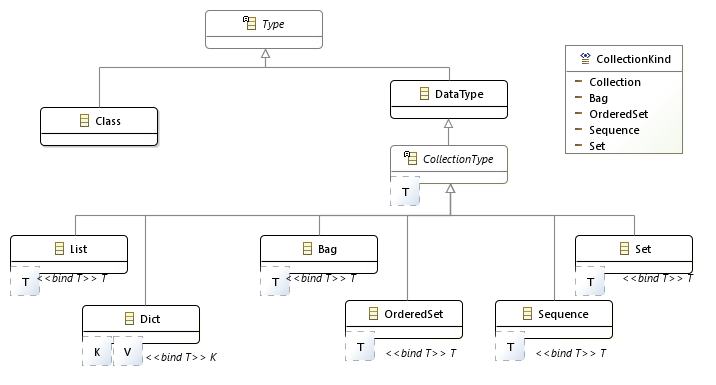
\includegraphics[width=1.0\textwidth]{Extensionsclassdiagram.png}
	\caption{CollectionType extensions.}
	\label{fig:Extensionsclassdiagram}
\end{figure}

Introduction of mutable types has bad consequences for facilities such as tracing that require a persisted value. In OCL, an immutable compound value is easily shared at very little cost by multiple consumers. In QVTo, a mutable compound value must be copied to avoid corruption. Since the copy may need to be a deep copy,  this may be very expensive, and worse since the deep copy may result in multiple copies of objects, it is not clear whether copied objects are equal to each other. Mutable types are not a natural extension of OCL.

Even at the modeling level mutable types create challenges. What is the correct metamodel relationship between a List and a Sequence? The QVT specification defines List and Dict as derived CollectionTypes and so their equality is determined by deep content comparison rather than simple object identity comparison appropriate for Class instances.

The extension of CollectionType undermines the expectation that all DataTypes (and CollectionTypes) are immutable. In particular the normal mechanism whereby DataType values are passed by value to operations or mappings fails. When a List is passed as an inout parameter it must be passed by reference in order for the DataType mutation to be passed back the caller. QVT 1.3 `solves' this by introducing a synthetic passed variable. There is strong case that List and Dict should be derivations of Class rather than CollectionType to reduce their OCL surprises.

Conclusion: QVTo's mutable CollectionTypes conflict with OCL.

\subsection{Mutable Expression Classes}
  
OCL defines a hierarchy of classes that extend OCLExpression, such as IfExp, PropertyCallExp, StringLiteralExp, VariableExp. These classes have a simple zero-or-more input, one output functionality that evaluates naturally as a side-effect free query.

OCLExpression is readily extended by other classes that also behave as side-effect free queries.

QVTr introduces a new TemplateExp hierarchy to support pattern matching. TemplateExp is defined as an OCLExpression and so syntactically may be used to write some rather challenging expressions. What does it mean for an iterator body to be a TemplateExp? In practice arbitrary expressions are not allowed by OCL. For instance the condition of an IfExp must be a Boolean expression, so we just need a clearer constraint on the permitted utility of TemplateExp.

Introduction of pattern matching expressions to OCL was discussed at the Aachen OCL workshop~\cite{aachen} and generally thought to be useful. These have very similar functionality to QVTr's template expressions and if introduced by OCL with a distinct syntax would cause a severe problem for QVTr; confusion through support for two alternative syntaxes or incompatibility through migration to the OCL syntax. A much better solution for QVTr is for OCL to use something very similar to the QVTr syntax, so that QVTr simplifies by re-using the syntax is promoted to OCL.

QVTc introduces an Assignment hierarchy to implement mutations. These exploit OCLExpression to define left and right hand sides of the assignment but do not extend OCLExpression; QVTc assignments do not encounter an OCL extension difficulty.

However, QVTo requires fine grained mutation and so a family of side-effecting ImperativeExpression classes such as AssignExp, BreakExp and ForExp are provided. ImperativeExpression extends OCLExpression allowing arbitrary use of side-effecting expressions within any OCLExpression. This would be a clear violation of OCL, but unfortunately it is so obvious that OCLExpressions are side effect free that the OCL specification does not specify that they are. Other languages make a clear distinction between clean Expressions and dirty Statements.  QVT 1.3 introduces a prohibition on the use of ImperativeExpression within non ImperativeExpression OCLExpressions. This goes most of the way to re-designating ImperativeExpression as a `Statement'; changing the inheritance should complete the clean-up.

Conclusion: QVTo's side-effecting ImperativeExpressions conflict with OCL.

\subsubsection{Complete Model}

A Complete OCL document provides additional class invariants, operations, properties that complement an existing metamodel; the additional facilities can be used as if they were part of the complemented metamodel. This is a very powerful capability, Classes are no longer closed; additional features may be added. Unfortunately the mechanisms by which closed UML classes become open OCL classes is unspecified. It is unclear whether a fully compliant implementation of open OCL classes is possible. The mechanism is therefore proprietary and not readily available for use by extensions.

Eclipse OCL~\cite{Eclipse-OCL} prototypes a solution whereby multiple packages with the same URI are logically merged as a CompletePackage containing the unmerged partial Packages. Within a CompletePackage, same-named Classes are logically merged as a CompleteClass containing the unmerged Classes.

Conclusion: One of OCL's most useful facilities is not extensible until properly specified.

\section{Structural Extension}\label{Structural Extension}

\subsection{Concrete Syntax}\label{Concrete Syntax}

The poor specification of OCL models and semantics has been accepted by the community since interchange occurs almost exclusively at the textual level where there is much less ambiguity. However even here, the lack of a clear `import' capability to identify the models in use makes the first couple of lines of many OCL documents proprietary. Similar problems apply to QVT.

The Concrete Syntax is specified by a grammar, or rather it should be. In the case of OCL, the grammar is partitioned into many small snippets with informal text to explain how ambiguities are to be resolved.

QVTc and QVTr provide grammars that appear to extend the OCL grammar. However since no coherent OCL grammar exists, QVTc and QVTr toolsmiths have to work much harder than should be necessary.

QVTo provides a complete grammar re-expressing parts of the OCL grammar in ways that do not obviously match the OCL snippets. In particular the additional ImperativeExpression clauses with similar syntaxes to OCL appear to displace some OCL functionality.

Conclusion: One day, a full exposition of the OCL grammar is probably extensible by QVTc and QVTr. It is not obvious that it would be extensible by an unchanged QVTo. 

\subsection{Standard Library}\label{Standard Library}

The OCL Standard Library defines useful types such as OclAny, Integer and Set(T), and useful operations such as OclAny::=(OclAny), Integer::div(Integer) and Set(T)::including(T) without which OCL would be unusable. OCL also provides powerful collection iterations, but until OCL 2.3 it was unclear whether the names of iterations were intrinsic to the OCL language, or an extension provided by the OCL Standard Library.

QVTc and QVTr, in QVT1.3, make no extensions to the OCL Standard Library.

QVTo defines a QVTo Standard Library that adds new types and operation and which extends the OCL StandardLibrary with further String operations.

Some of the original QVTo 1.0 extensions, such as String::+(String) were adopted by OCL 2.2.

The OCL Standard Library is no more than words in the specification and QVTo can easily extend this informality.

True extensibility requires that OCL define its library as a model in a form that supports QVTo to define its library as an extending model. Eclipse OCL provides an OCL library model that is currently extended by small Eclipse QVTc/QVTr~\cite{Eclipse-QVTd}library models. These models rely on the ability of a pivot model to merge class and operation declarations from diverse sources.

\subsubsection{allInstances}

OclElement::allInstances() is an interesting operation that is sometimes discouraged in OCL because it poses implementation challenges. For QVT 1.3 addressed the further challenges:

\begin{itemize}
\item which of the input/intermediate/output models contribute instances?
\item how does the functionality accommodate mutation of objects?  
\end{itemize}

QVTo introduces a Model::objectsOfKind operation to resolve the first question explicitly. Since QVTo supports fine-grained mutation, the result represents the prevailing state. allInstances() returns the prevailing state of all instances in all models.

The prevailing state is not a very useful concept for QVTc or QVTr for which there is only a single giant mutation. Neither of the initial or final states are well-defined for the case of a composed cascade of QVTc or QVTr transformations and so for QVTc and QVTr allInstances is restricted to the final state of the input/intermediate/output model within which allInstances is invoked.

Conclusion: allInstances(), as specified, is not extensible to QVT. Improved wording of the OCL specification might extrapolate better. 

\subsection{Abstract Syntax}\label{Abstract Syntax}

The Abstract Syntax model is arguably the most important part of the OCL language since it defines the boundary between development by the OCL programmer and the subsequent execution by an OCL enabled application. For QVT, this is even more important since the AS is the executable transformation.

The QVTr and QVTc AS extend EMOF and OCL without undue difficulty, although the design decision that Transformation extends both Class and Package breaks the expectation that the container of an Operation is not a Package.

QVTo has similar anomalies with Module. Much more difficulty arises in regard to contextual operations and properties. Logically these contextual facilities mirror Complete OCL's ability to define and extend classes, but since the details of this ability are unspecified, they cannot be re-used by QVTo, which is therefore forced to provide yet another family of modeling classes that also poses challenges in providing valid objects for OperationCallExp::referredOperation or PropertyCallExp::referredProperty to reference.

Conclusion: the OCL AS is difficult to extend since important OCL capabilities are missing from the hints in the OCL specification.    

\subsubsection{CollectionType::kind}

OCL defines a family of concrete Bag, OrderedSet, Sequence, Set types that extend the abstract Collection type. These are amenable to further extension by inheritance. However OCL also specifies a CollectionType::kind property using the closed CollectionKind enumeration of Collection, Bag, OrderedSet, Sequence, Set. Any use of CollectionType::kind is readily replaced by oclIsTypeOf, so CollectionType::kind can be usefully removed eliminating the unnecessary prohibition on additional collection types such as QVTo's List and Dict types. 

\subsubsection{Operation::isVirtual}

The semantics of operation overloading are undefined for OCL, although there seems to be general agreement~\cite{aachen} that something similar to Java semantics is appropriate.

QVTo introduces an ImperativeCallExp::isVirtual property that highlights a deficiency in OCL's OperationCallExp. How can virtual dispatch be suppressed? In the concrete syntax, one might expect that a.b() invokes the most derived overload of b() applicable to the actual type of a. In contrast a.B::b() might be expected to invoke precisely B::b() even if B::b() is not the most derived overload. Promotion of ImperativeCallExp::isVirtual to OperationCallExp::isVirtual solves the problem.

Conclusion: QVTo successfully extends OCL by providing a bug fix.

\subsubsection{Multiple operation returns}

The semantics of a multi-valued operation return are undefined for OCL, since superficially OCL only supports a single return. However OCL aspires to UML alignment and UML supports multiple returns.

QVTo supports directional parameters (in/inout/out) and so the challenge of multi-valued returns cannot be ignored. QVTo solves the problem by specifying a Tuple so that the multiple values are returned as one. OCL should endorse this approach. 

Conclusion: QVTo successfully extends OCL by providing a bug fix.

\subsection{Validation}\label{Validation}

The validation provided by Well-Formedness Rules does not always extend well. For instance UML defines that NamedElements within a Namespace are distinguishable, but the Constraint class is a NamedElement and numerous OCL examples leave the Constraint name blank. Is the name left blank, violating the UML distinguishability validation, or is tooling required to synthesize unambiguous names?

An alternative solution is to define validation constraints with loopholes. UML therefore defines that the Namespace::members\_distinguishable invariant is computed by the Namespace::membersAreDistinguishable() operation. The Namespace operation invokes  NamedElement::isDistinguishableFrom(). This provides a loophole in Namespace, through overloading of membersAreDistinguishable, and in NamedElement, through overloading isDistinguishableFrom. But Constraint does not exploit the loophole opportunity leaving typical OCL usage in breach of UML.

The OCL WFRs are very immature in terms of their live usage in real OCL tools. They are pretty much untested with respect to use by extending tools. Consequently the loopholes to support extensibility are missing.

One example of a missing loophole occurs for a Variable which in OCL expects its initializer to be type conformant to the variable. However in a transformation language, a similar usage may represent a predicate whereby a type mismatch is not a compile-time error, rather it is a run-time test guarding a mapping execution for use only when the actual argument is type conformant at run-time.

Alternatively the lack of the loophole demonstrates a flaw in the QVT re-use of Variable. If QVT needs to change the semantics of Variable, QVT should introduce a GuardVariable for the changed semantics. This is comparatively easy once the under-specification of the VariableDeclaration class is completed. It may even be worth introducing IteratorVariable and LetVariable to clarify their distinct initialization semantics.


\begin{figure}[h]
	\centering
	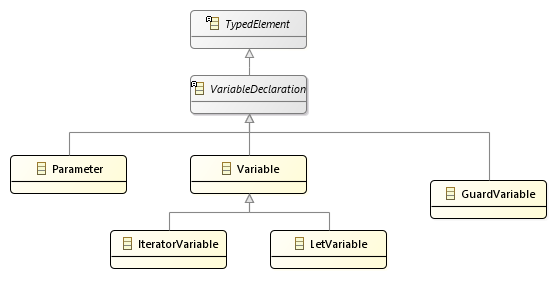
\includegraphics[width=1.0\textwidth]{Variablesclassdiagram.png}
	\caption{Variable classes.}
	\label{fig:Variablesclassdiagram}
\end{figure}

Conclusion: OCL WFRs need revision or observance to support extensibility.

\section{Tooling}\label{Tooling}

If OCL is to be easily extended, OCL tools must be similarly easily extended, either be using an inherently extensible implementation or by auto-generating the implementation from some extensible abstraction.

Today's tools are inherently extensible only if you are a skilled Java programmer with time to spare. It is not obvious that this approach can be dramatically improved. However auto-generation is steadily improving. Figure~\ref{Tooling} shows the typical components that an OCL or QVT tool requires. The top row shows metamodels, grammars and rules that should be defined by the language specification. The bottom rows show the corresponding tool representations as squares and conversions as lozenges. Tooling such as EMF auto-generates useful Java from UML-like Ecore models for Concrete Syntax Tree and Abstract Syntax Graph. Eclipse OCL's OCLinEcore enables the models to be enriched with OCL operation bodies and property values and so generate Java code for a Validator. Tools such as Xtext can auto-generate Lexer, Parser and Editor from annotated EBNF grammars. Eclipse OCL provides an Xtext editor specifically customized to editing extensible library models. 
Most areas of OCL tooling are therefore amenable to auto-generation from models and grammars and so re-auto-generation for extended models and grammars.  There are however two challenging area.

\begin{figure}[h]
	\centering
	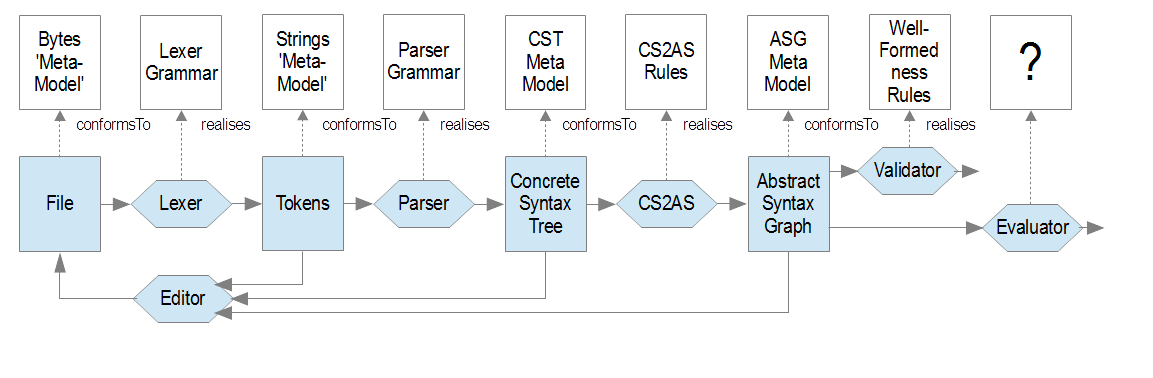
\includegraphics[width=1.0\textwidth]{Tooling.png}
	\caption{Tooling.}
	\label{fig:Tooling}
\end{figure}

\subsection{CS2AS}

The Xtext tooling can auto-generate a parser for a model that resembles the Concrete Syntax (CS), but this has significant differences to that specified as the OCL Abstract Syntax (AS). A CS2AS mapping is therefore required, and since OCL has some unpleasant ambiguities and some non-trivial rules such as implicit source for locating names, additional complexities arise in the CS2AS mapping. This challenge is being addressed with a DSL that defines the mappings, disambiguations and lookups \cite{cs2as}. 

Once CS2AS tooling is in place the semi-formality of OCL's Clause 9 can be replaced by a DSL model from which tooling and specification are auto-generated. Bug fixing for the tolling will automatically bug fix the specification. Extension of the DSL model can provide similar benefits for QVTc and QVTo that have no CS2AS specification at all and for QVTr that has a very suspect specification.

The DSL model for CS2AS should complement the CS model, AS model, library model and language grammar to support auto-generation of compile-time tooling.

\subsection{Evaluation}

Interpreters and code generators for OCL are currently hand-crafted and although there have been many attempts to formalize OCL semantics, these efforts such as the recent FeatherWeight OCL~\cite{FeatherweightOCL} concentrate on proofs rather than utility.

Today's hand-crafted code can, in principle, be replaced by auto-generated code from a suitable abstraction. Identifying this abstraction and attempting to correlate it with and perhaps even auto-generate it from provable semantics remains a topic for future work.

\subsection{Modules}

The OCL language provides some core functionalities such as simple arithmetic (Boolean, Integer, String), simple expressions (if, let), operation calls and model navigation. Further functionalities such as reals, templates, collections, iterations, tuples, patterns, states and messages are increasingly specialized and not required by all users. Support for each of these functionalities may require grammar, concrete syntax, abstract syntax, disambiguation, libraries and evaluation implementation contributions. Support for an additional functionality such as time may again require many of the same implementation contributions.

Currently all OCL functionalities are specified and implemented as a monolith inhibiting the use of a lighter weight OCL or of an extended OCL. If each non-core functionality is separately specified as a distinct module and if tooling can be auto-generated from each module, users can create a lighter weight OCL and / or add additional modules for an extended OCL.

A module therefore needs to provide a number of partial contribution to each functionality. 

\subsubsection{Partial Grammar}
Most tools expect full grammars and provided limited extension capabilities. New tooling may be required to weave partial grammars together.

\subsubsection{Partial CS and AS Models}
Partial models are not normally supported, however technologies such as UML's Package merge of OCL's Complete Models allow multiple models to be treated as a composite model.

\subsubsection{Partial Libraries}
The Eclipse OCL Library model is just a DSL for a conventional model. Operations may be specified with OCL bodies or redirected to a custom Java implementation.

\subsubsection{Partial CS2AS}
The CS2AS is a new development. Support for partial contributions has been considered.

\subsubsection{Partial Evaluation}
No auto-generation is currently available. Perhaps implementation stubs could be provided to minimize user activity until a better auto-generation is available.

\section{Related Work}\label{Related Work}

OCL was considered as part of a Family of Languages in \cite{OCLFamily} which also concluded that the current exposition of the OCL specification hinders its re-use.

Time forms an important part of the specification of Real-Time systems, but OCL has no support for time. Many extensions of OCL have therefore appeared that remedy this deficiency \cite{TemporalOCL3}\cite{TemporalOCL1}\cite{TemporalOCL4}\cite{TemporalOCL2}.

QVTo is not the only imperative extension of OCL. The  Simple OCL-based Imperative Language (SOIL) \cite{SOIL} is used in a much more disciplined and restricted fashion within USE \cite{USE}. It avoids the mistake of confounding side-effecting statements with side-effect free expressions.

Some implementations of OCL deliberately deviate from the standard. For instance Epsilon OCL \cite{Epsilon} discards the distinction between collection (arrow) and object (dot) navigation operators. This should certainly be possible in the interests of ergonomic research. Other implementations of OCL accidentally deviate variously because the specification cannot be understood and because the implementers fail to study the specification with sufficient care.
%
\section{Conclusions}\label{Conclusions}
%
We have described how accurate models underlying OCL do not exist and so OCL is not extensible with respect to its models.

We have described how a clear specification for OCL does not exist and so OCL is not extensible with respect to its specification.

However, since much of the functionality of OCL is `obvious', we have shown how the principles of OCL can be successfully extended and re-used in practice.

For QVTc and QVTr we find that the extension works well.

For QVTo we find non-trivial conflicts with OCL that are aggravated by some poor language design decisions. It would be much better for QVTo to use rather than extend OCL.

%\paragraph{Acknowledgments}

%Many thanks to Adolfo S\'{a}nchez-Barbudo Herrera for his detailed review and constructive comments.

%
% ---- Bibliography ----
%
\begin{thebibliography}{}
%
\bibitem{OCLFamily}
Akehurst, D., Howells, G., McDonald-Maier, K.: Supporting OCL as part of a Family of Languages. ... 2005

\bibitem{aachen}
Brucker, A., Chiorean, D., Clark, T., Demuth, B., Gogolla, M., Plotnikov, D., Rumpe, B., Willink, E., Wolff, B.:
Report on the Aachen OCL Meeting .
CEUR-WS Proceedings, Vol-1092 (2013)
\url{http://ceur-ws.org/Vol-1092/aachen.pdf}

\bibitem{FeatherweightOCL}
Brucker, A., Tuong, F., Wolff, B.: Featherweight OCL:  A Proposal for a Machine-Checked Formal Semantics for OCL 2.5, \url{https://www.isa-afp.org/entries/Featherweight\_OCL.shtml}

\bibitem{SOIL}
B\~uttner, F., Gogolla, M.: Modular Embedding of the Object Constraint Language into a Programming Language,
14th Brazilian Symposium on Formal Methods, Foundations and Applications SBMF 2011, Sptember 2011.

\bibitem{TemporalOCL3}
Conrad, s.,  Turowski, K.: Temporal OCL Meeting Specification Demands for Business Components.
In Unified modeling language: systems analysis, design and development issues IGI Publishing Hershey, PA, USA, 2001.

\bibitem{TemporalOCL1}
Kanso, B., Taha, S.: Towards Temporal constraint Support for OCL.
5th International Conference of Software Language Engineering, SLE 2012

\bibitem{Epsilon}
Kolovos, D., Rose, L., Garc\'ia-Dom\'inguez, A., Paige, R.: The Epsilon Book, \url{https://git.eclipse.org/c/epsilon/org.eclipse.epsilon.git/plain/doc/
org.eclipse.epsilon.book/EpsilonBook.pdf}

\bibitem{cs2as}
S\'anchez-Barbudo Herrera, A., Willink, E., Paige, R.: Domain Specific Transformation Language to Bridge Concrete and Abstract Syntax,  9th International Conference Theory and Practice of Model Transformations (ICMT 2016), Vienna, 2016 

\bibitem{TemporalOCL4}
Soden, M., Eichler, H.: Temporal Extensions of OCL Revisited.
5th European Conference, ECMDA-FA 2009, Enschede, The Netherlands, 2009.

\bibitem{TemporalOCL2}
Ziemann, P.,  Gogolla, M.: OCL  Extended  with  Temporal  Logic. 
5th International Andrei Ershov Memorial Conference, Perspectives of System Informatics 2003.

\bibitem{Eclipse-EMF}
Eclipse EMF Project.\\
\url{https://projects.eclipse.org/projects/modeling.emf.emf}

\bibitem{Eclipse-OCL}
Eclipse OCL Project.\\
\url{https://projects.eclipse.org/projects/modeling.mdt.ocl}

\bibitem{Eclipse-QVTd}
Eclipse QVT Declarative Project.\\
\url{https://projects.eclipse.org/projects/modeling.mmt.qvtd}

\bibitem{QVT-1.3}
OMG. Meta Object Facility (MOF) 2.0 Query/View/Transformation Specification, Version 1.3.
OMG Document Number: ptc/16-06-03, June 2016.

\bibitem{UML-2.5}
OMG Unified Modeling Language (OMG UML), Version 2.5, {OMG Document Number}: formal/15-03-01, Object Management Group (2015), \url{http://www.omg.org/spec/UML/2.5}

\bibitem{OCL-2.4}
Object Constraint Language. Version 2.4., OMG Document Number: formal/2014-02-03, Object Management Group (2009),  \url{http://www.omg.org/spec/OCL/2.4}

\bibitem{USE}
USE, The UML-based Specification Environment \url{http://useocl.sourceforge.net/w/index.php/Main\_Page}
\end{thebibliography}
\end{document}
